%==========================================================
% Capitulo 2: Revisao Bibliografica.
% 
% Autor
% Heitor Luis Polidoro
% 
% Orientador
% Prof. Dr. Denis Fernando Wolf
%==========================================================

\chapter{Revisão Bibliográfica}
\label{revisao_bibliografica}
TEM QUE ARRUMAR A SEQÜÊNCIAS DAS SESSÕES

\section{Controle do Robô}
\label{controle_do_robo}
O controle do robô será desenvolvido utilizando-se a biblioteca Player/Stage \cite{Gerkey2003}, a qual permite que sejam realizadas simulações antes que os algoritmos sejam testados com o robô real (Figura \ref{fig:gazebo_pioneer}). Essas simulações são importantes para o aperfeiçoamento dos parâmetros, como distâncias, velocidades, etc, antes do teste no Pioneer.

\begin{figure}[ht]
	\centering
	\subfigure[Gazebo]{
		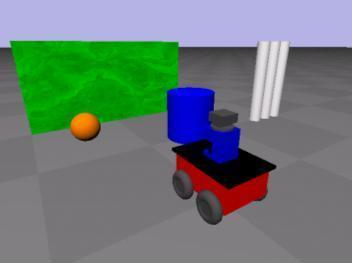
\includegraphics[width=0.55\textwidth]{../imagens/gazebo.jpg}
		\label{fig:gazebo}}
	\subfigure[Pioneer]{
		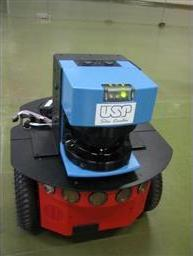
\includegraphics[width=0.35\textwidth]{../imagens/pioneer.jpg}
		\label{fig:pioneer}}
	\caption{Robô Pioneer, Simulado e Real.}
	\label{fig:gazebo_pioneer}
\end{figure}

\subsection{Player}
\label{player}
O Player é um servidor de rede para controlar robôs. Executando embarcado no robô, o Player provê uma interface simples e clara dos sensores e atuadores do robô sobre uma rede IP. O programa cliente ``conversa'' com o Player utilizando sockets TPC, lendo dados dos sensores, escrevendo comandos nos atuadores e configurando dispositivos em tempo de execução.
O servidor Player foi desenvolvido para ser independente de linguagem e de plataforma. O programa cliente pode executar em qualquer máquina que tenha conexão de rede com o robô, e pode ser escrito em qualquer linguagem que suporte sockets TCP. Atualmente existem clientes disponíveis em C++, Tcl, Java em Phyton \cite{Player}. Futuramente, o Player não fará suposições sobre como o programa de controle do robô é estruturado, ou seja, poderá-se escrever desde programas multi-threads altamente concorrentes até programas seqüências simples.

\subsection{Stage}
\label{stage}
O Stage é usado normalmente como um plugin para o Player, provendo uma série de dispositivos virtuais para os clientes Player. Os usuários escrevem as rotinas e algoritmos normalmente, como clientes para um servidor Player. Não é possível para clientes distinguir a diferença entre os dispositivos reais do robô e os equivalentes simulados pelo Player/Stage. Com isso clientes Player desenvolvidos usando o Stage precisarão de pouca ou nenhuma modificação para trabalhar com o robô real, e vice-versa. Em muitos casos basta somente mudar no cliente o endereço IP de onde está o servidor. O Stage também pode simular uma população de robôs móveis, sensores e objetos num ambiente bi-dimensional (Figura \ref{fig:stage}) \cite{Player}. Neste projeto será utilizado somente um robô e o sensor LASER.

\figura{../imagens/stage.jpg}{.5}{Simulação com 5 robôs, 2 objetos, LASER, sonar e blobfinder.}{fig:stage}




